\documentclass{beamer}


\usepackage{graphicx}
\usepackage{hyperref}
\usepackage{minted}


\title{Fun with Generics}
\author{Benjamin Hodgson}
\date{17th September 2015}


\begin{document}
  \frame{\titlepage}

  \begin{frame}[fragile]
    \frametitle{Example 1: FileStore}
    \begin{minted}{csharp}
interface IFileStore
{
    Stream Read(IPathKey key);
    void Write(IPathKey key, Stream stream);
}
    \end{minted}
\end{frame}

  \begin{frame}[fragile]
    \begin{minted}{csharp}
class FileSystemFileStore : IFileStore
{
    IFileSystemPathGenerator _generator;
    IFileSystemReader _reader;
    IFileSystemWriter _writer;
    
    public Stream Read(IPathKey key)
    {
        string absolutePath = _generator.Generate(key);
        return _reader.Read(absolutePath);
    }
    public void Write(IPathKey key, Stream stream)
    {
        string absolutePath = _generator.Generate(key);
        _writer.Write(absolutePath, stream);
    }
}
    \end{minted}
\end{frame}

  \begin{frame}[fragile]
    \begin{minted}{csharp}
class AwsFileStore : IFileStore
{
    IAwsKeyGenerator _keyGenerator;
    IAwsReader _reader;
    IAwsWriter _writer;

    public Stream Read(IPathKey key)
    {
        S3Key ey = _keyGenerator.Generate(key);
        return _reader.Read(key);
    }
    public void Write(IPathKey key, Stream stream)
    {
        S3Key key = _keyGenerator.Generate(key);
        _writer.Write(key, stream);
    }
}
    \end{minted}
\end{frame}

  \begin{frame}[fragile]
    \begin{minted}{csharp}
class RackspaceCloudFileStore : IFileStore
{
    IRackspaceContainerNameGenerator _cGenerator;
    IRackspaceObjectPathGenerator _pathGenerator;
    IRackspaceReader _reader;
    IRackspaceWriter _writer;
    public Stream Read(IPathKey key)
    {
        string containerName = _cGenerator.Generate(key);
        string objectPath = _pathGenerator.Generate(key);
        return _reader.Read(containerName, objectPath);
    }
    public void Write(IPathKey key, Stream stream)
    {
        string containerName = _cGenerator.Generate(key);
        string objectPath = _pathGenerator.Generate(key);
        _writer.Write(containerName, objectPath, stream);
    }
}
    \end{minted}
\end{frame}

  \begin{frame}[fragile]
    \begin{minted}{csharp}
interface IPathGenerator<out TPath>
{
    TPath Generate(IPathKey key);
}
interface IFileReader<in TPath>
{
    Stream Read(TPath path);
}
interface IFileWriter<in TPath>
{
    void Write(TPath path, Stream stream);
}
    \end{minted}
    And:
    \begin{minted}{csharp}
class RackspacePath
{
    public string ContainerName { get; set; }
    public string ObjectPath { get; set; }
}
    \end{minted}
\end{frame}

  \begin{frame}[fragile]
    \begin{minted}{csharp}
class FileStore<TPath> : IFileStore
{
    IPathGenerator<TPath> _pathGenerator;
    IFileReader<TPath> _reader;
    IFileWriter<TPath> _writer;
    
    public Stream Read(IPathKey key)
    {
        TPath path = _pathGenerator.Generate(key);
        return _reader.Read(path);
    }
    public void Write(IPathKey key, Stream stream)
    {
        TPath path = _pathGenerator.Generate(key);
        _writer.Write(path, stream);
    }
}
    \end{minted}
\end{frame}

  \begin{frame}
    \frametitle{Variance}
    When is a generic type a subtype of another generic type?
    \begin{center}
    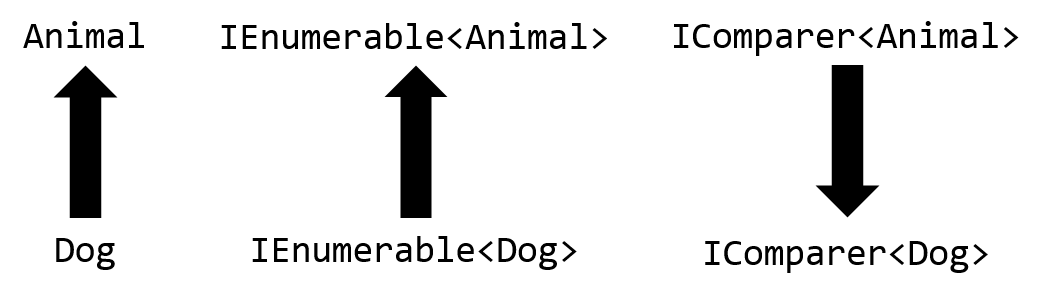
\includegraphics[scale=0.5]{variance.png}
    \end{center}
    \begin{itemize}
      \item \texttt{IList<T>} is \emph{invariant}
      \begin{itemize}
        \item An \texttt{IList} is never a subtype of another \texttt{IList}
        \item \texttt{T} appears in both \emph{input} and \emph{output} positions
      \end{itemize}
      \item \texttt{IEnumerable<out T>} is \emph{covariant}
      \begin{itemize}
        \item \texttt{IEnumerable}'s subtyping relation goes in the \emph{same direction} as the type parameter
        \item \texttt{IEnumerable} \emph{produces} \texttt{T}s
      \end{itemize}
      \item \texttt{IComparer<in T>} is \emph{contravariant}
      \begin{itemize}
        \item \texttt{IComparer}'s subtyping relation goes in the \emph{opposite direction} to the type parameter
        \item \texttt{IComparer} \emph{consumes} \texttt{T}s
      \end{itemize}
    \end{itemize}
  \end{frame}

  \begin{frame}[fragile]
    \frametitle{Variance}
    \begin{minted}{csharp}
float AverageAge(IEnumerable<Animal> animals)
{
    return animals.Select(a => a.Age).Sum()
           / animals.Count();
}
AverageAge(new List<Dog> { rex, fido, richard });
    \end{minted}
    \pause
    \begin{minted}{csharp}
bool DogIsBetter(IComparer<Dog> comparer)
{
    return comparer.Compare(this.dog1, this.dog2) > 0;
}
DogIsBetter(new AnimalComparer());
    \end{minted}
    \pause
    \begin{minted}{csharp}
void AddGiraffe(IList<Animal> animals)
{
    animals.Add(new Giraffe());
}
// AddGiraffe(new List<Dog>());
    \end{minted}
\end{frame}
  
  \begin{frame}
    \centering
    
\includegraphics[scale=0.3]{science.jpg}
  \end{frame}
  
  \begin{frame}
    \frametitle{The Spectrum...}
    
    \begin{itemize}
      \item ... of Safety
      \item ... of Usability
      \item ... of Power
      \item ... of Flexibility
    \end{itemize}
    \vfill
    \centering
    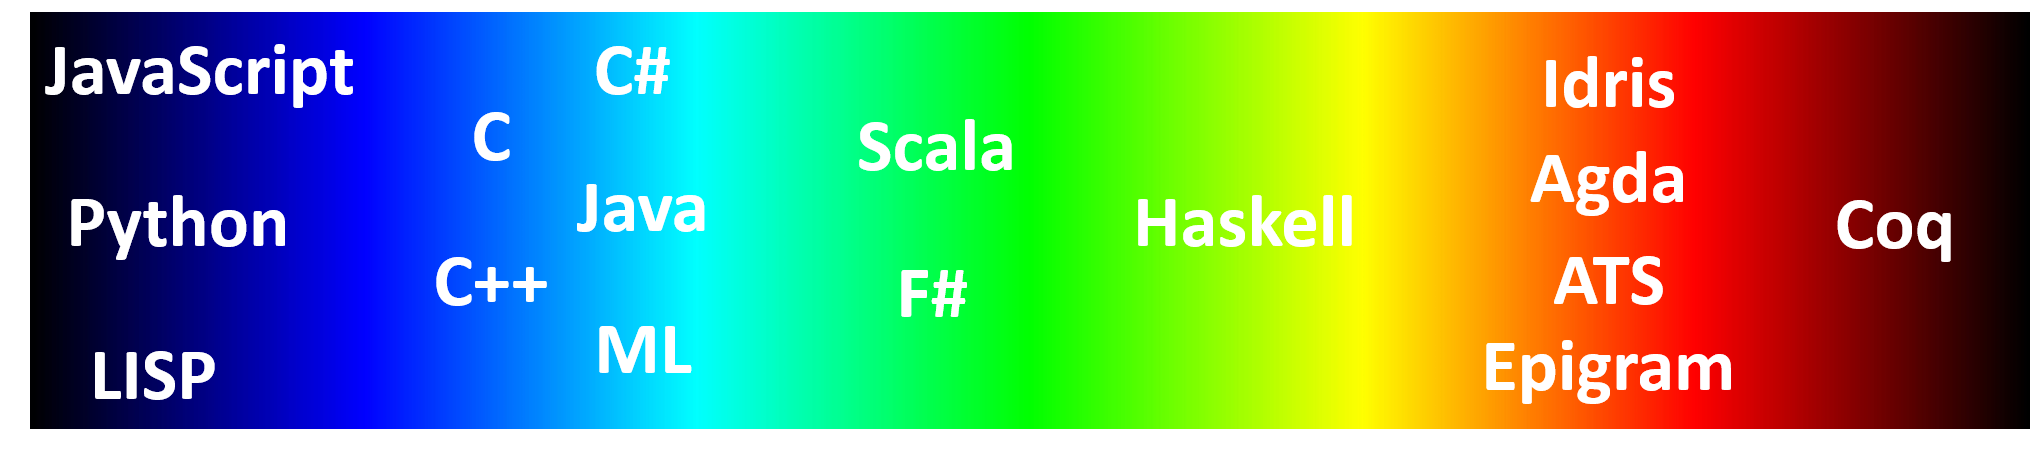
\includegraphics[scale=0.3]{spectrum.png}
  \end{frame}

  \begin{frame}[fragile]
    \frametitle{Example 2: Permissions Engine}
    \emph{Specifications}: small classes testing something about an object, and a way to combine them.
    
    \begin{minted}{csharp}
interface ISpecification<in T>
{
    bool IsSatisfiedBy(T candidate);
}
    \end{minted}
    \pause
    \begin{minted}{csharp}
var context = new BlogContext
{
    CurrentUser = user,
    BlogPost = post
}
if (!userCanCommentOnBlogPost.IsSatisfiedBy(context))
{
    throw new PermissionException(
        "You can't comment on that post"
    );
}
    \end{minted}
\end{frame}
    
  \begin{frame}[fragile]
    Represent combinations of specifications as a syntax tree.
    \frametitle{Example 2: Permissions Engine}
    \begin{center}
    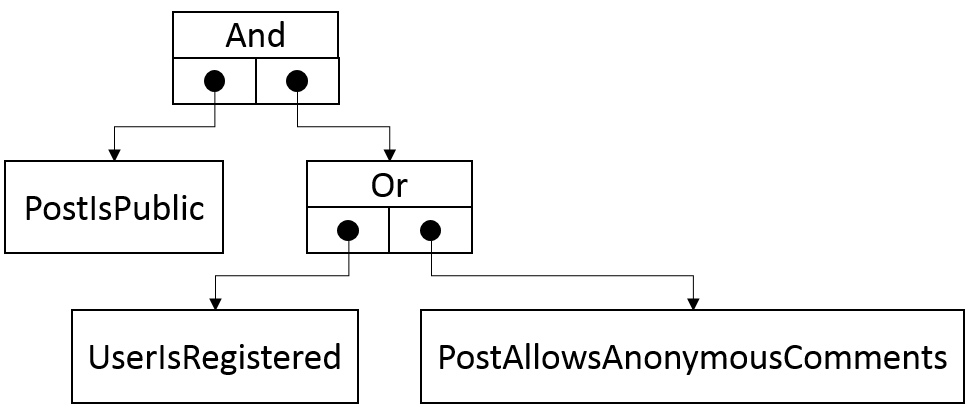
\includegraphics[scale=0.6]{specification.png}
    \end{center}
    
    \begin{minted}{csharp}
var userCanCommentOnBlogPost =
  new AndSpecification<BlogContext>(
    new PostIsPublic(),
    new OrSpecification<BlogContext>(
      new UserIsRegistered(),
      new PostAllowsAnonymousComments()
    )
);
    \end{minted}
\end{frame}

  \begin{frame}[fragile]
    \frametitle{Example 2: Permissions Engine}
    \begin{minted}{csharp}
interface ISpecificationVisitor<T, out TReturn>
{
    TReturn Visit(LeafSpecification<T> spec);
    TReturn Visit(AndSpecification<T> spec);
    TReturn Visit(OrSpecification<T> spec);
    TReturn Visit(NotSpecification<T> spec);
}
interface ISpecification<T>
{
    TReturn Accept<TReturn>(
        ISpecificationVisitor<T, TReturn> visitor);
}
    \end{minted}
\end{frame}

  \begin{frame}[fragile]
    \frametitle{Problem}
    Code duplication because \texttt{void} is not a real type
    
    \begin{minted}{csharp}
interface ISpecificationVisitor<T>
{
    void Visit(LeafSpecification<T> spec);
    void Visit(AndSpecification<T> spec);
    void Visit(OrSpecification<T> spec);
    void Visit(NotSpecification<T> spec);
}
    \end{minted}
    
    Alternatively, a type that means the same as \texttt{void}:
    
    \begin{minted}{csharp}
sealed class Unit
{
    private static readonly Unit _default = new Unit();
    private Unit() { }
    public Unit Default { get { return _default; } }
}
    \end{minted}
\end{frame}

  \begin{frame}[fragile]
    \frametitle{Problem}
    Why isn't \texttt{ISpecification<T>} contravariant?
    A specification which tests fruit should work when you need to test an apple.
    
    \begin{minted}{csharp}
class FruitIsRipe : ISpecification<Fruit> { /* ... */ }
void TestApple(ISpecification<Apple> spec);
    \end{minted}
    
    \begin{itemize}
      \item \texttt{ISpecificationVisitor<T, TReturn>} would have to be \emph{co}variant in \texttt{T}
      \item \texttt{LeafSpecification<T>}, \texttt{AndSpecification<T>} etc would have to be \emph{contra}variant
      \item Classes can never be variant in C$\sharp$
      \item You have to make an interface for every class!
    \end{itemize}
\end{frame}

  \begin{frame}
    \centering
    
\includegraphics[scale=0.6]{AngryBaby.jpg}
  \end{frame}

  \begin{frame}
    \frametitle{Two kinds of polymorphism}
    \begin{table}[h]
      \begin{tabular}{ll}
        \hline
        \textbf{Parametric polymorphism} & \textbf{Subtype polymorphism} \\ \hline
        Lots of generality               & Only works with subtypes      \\
        Requires design-time foresight   & Ad-hoc extensibility          \\ \hline
      \end{tabular}
    \end{table}
    \centering
    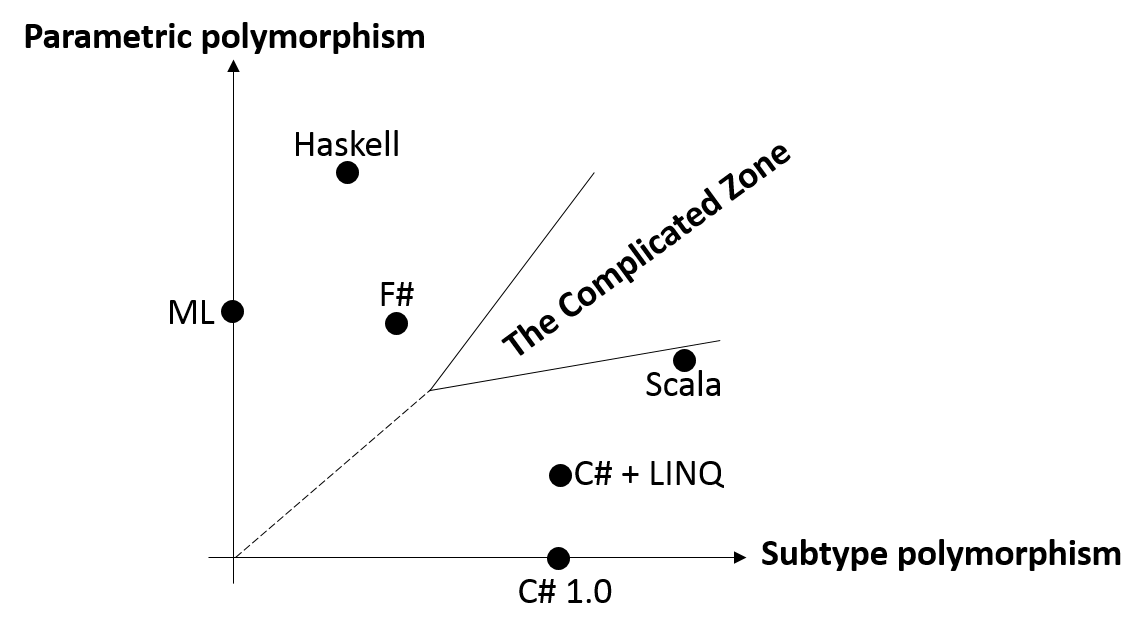
\includegraphics[scale=0.6]{polymorphismaxes.png}
  \end{frame}

  \begin{frame}[fragile]
    \frametitle{Example 3: Test Data Builders}
    \begin{itemize}
      \item A simple tool to make it easy to set up test data -- everything gets a default, which can be overridden if the test needs it.
      \item Imagine testing a the \texttt{SalaryPayment} class of a payroll system
      \begin{itemize}
        \item When \emph{building}, the recipient of a payment gets a default value
        \item When \emph{saving}, you have to set the recipient -- it must be a \emph{real} \texttt{Employee} to satisfy the foreign key
      \end{itemize}
    \end{itemize}
        
    \begin{minted}{csharp}
new PaymentTestDataBuilder()
    .WithRecipient(employee)
    .Save();  // fine
new PaymentTestDataBuilder()
    .Build();  // fine
new PaymentTestDataBuilder()
    .Save();  // runtime exception!
    \end{minted}
\end{frame}

  \begin{frame}[fragile]
    \frametitle{Attempt 1: Subclass}
    \begin{minted}{csharp}
class PaymentTestDataSaver : PaymentTestDataBuilder
{
    public PaymentTestDataSaver(Employee recipient)
    { /* ... */ }
    public SalaryPayment Save()
    { /* ... */ }
}

new PaymentTestDataSaver(employee)
    .Save();  // :)
new PaymentTestDataSaver(employee)
    .WithDateIssued(new DateTime(2015, 9, 17))
    .Save();  // compile error :(
    \end{minted}
    
    The declared return type of \texttt{WithPaymentDate} is \texttt{SalaryPaymentTestDataBuilder}.
\end{frame}

  \begin{frame}[fragile]
    \frametitle{Attempt 2: Parameterise the hierarchy}
    \textbf{Idea}: Parametrise the return type and specialise in the subclasses.
    Use \emph{F-bounds} to constrain the return type to be ``the type of \texttt{this}''.
    \begin{minted}{csharp}
abstract class PaymentTestDataBuilder<TSelf>
    where TSelf : PaymentTestDataBuilder<TSelf>
{
    public TSelf WithRecipient(Employee recipient)
    {
        // ...
        return This();
    }
    public TSelf WithDateIssued(DateTime date)
    {
        // ...
        return This();
    }
    protected abstract TSelf This();
}
    \end{minted}
\end{frame}

  \begin{frame}[fragile]
    \frametitle{Attempt 2: Generic base class}
    \begin{minted}{csharp}
class PaymentTestDataBuilder :
    PaymentTestDataBuilder<PaymentTestDataBuilder>
{
    protected override PaymentTestDataBuilder This()
    { return this; }
}
class PaymentTestDataSaver :
    PaymentTestDataBuilder<PaymentTestDataSaver>
{
    public PaymentTestDataSaver(Employee recipient)
    { /* ... */ }
    protected override PaymentTestDataSaver This()
    { return this; }
    public SalaryPayment Save() { /* ... */ }
}
    \end{minted}
\end{frame}

  \begin{frame}[fragile]
    \frametitle{Problems}
    F-bounds aren't quite strong enough.
    \begin{minted}{csharp}
class PathologicalBuilder
                            // Not the type of this!
    : PaymentTestDataBuilder<PaymentTestDataSaver>
{
    // ...
}
    \end{minted}
    
    Once you have one valid subclass, you can add invalid subclasses to your heart's content.
    F-bounds are not \emph{quite} strong enough to express self-types.
\end{frame}

  \begin{frame}
    \centering
    
\includegraphics[scale=0.8]{nic.png}
  \end{frame}

  \begin{frame}[fragile]
    \frametitle{Attempt 3: Type-level data}
    \textbf{Idea}: use \emph{phantom types} to represent validity
    \begin{minted}{csharp}
sealed class True { }
sealed class False { }

class PaymentTestDataBuilder<HasRecipient>
{
  public PaymentTestDataBuilder<True>
        WithRecipient(Employee recipient)
  {
    return new PaymentTestDataBuilder<True>
        (recipient);
  }
}
    \end{minted}
\end{frame}

  \begin{frame}[fragile]
    \frametitle{Attempt 3: Type-level data}
    \begin{minted}{csharp}
class PaymentTestDataBuilder
    : PaymentTestDataBuilder<False>
{ }

static class TestDataBuilderExtensions
{
    public SalaryPayment Save(
        this PaymentTestDataBuilder<True> builder)
    {
        // ...
    }
}
    \end{minted}
\end{frame}

  \begin{frame}
    \centering
    
\includegraphics[scale=0.3]{brain_melt_2.jpg}
  \end{frame}

  \begin{frame}[fragile]
    \frametitle{Example 4: Vectors}
    The classic toy example of dependent types: a sequence with static knowledge of how long it is.
    
    \textbf{Idea}: Write a phantom type representing lengths.
    Increment this phantom type every time you add an element to a vector.
    Later, check whether the length type parameter is greater than 1.
    
    \pause
    \vfill
    How to represent numbers in the type system?
    Mathematicians define natural numbers inductively:
    \begin{enumerate}
      \item $0$ is a natural number.
      \item For every natural number $n$, the \emph{successor} of $n$, $S(n)$, is a natural number.
    \end{enumerate}
    \begin{minted}{csharp}
sealed class Z { }  // Z for Zero
sealed class S<N> { }  // S for Successor
    \end{minted}
    
    $0 \leftrightarrow$ \texttt{Z}
    
    $1 \leftrightarrow$ \texttt{S<Z>}
    
    $2 \leftrightarrow$ \texttt{S<S<Z>>}
    
    $3 \leftrightarrow$ \texttt{S<S<S<Z>>>}
\end{frame}

  \begin{frame}
    \frametitle{Linked list recap}
    \begin{itemize}
      \item Two cases: \texttt{Nil} and \texttt{Cons}.
      \begin{itemize}
        \item \texttt{Nil} contains no elements.
        \item \texttt{Cons} contains one element and a pointer to the rest of the list.
      \end{itemize}
      \item Represent each case as a class.
    \end{itemize}
    \texttt{[3,2,1]} $\leftrightarrow$ \texttt{new Cons(3, new Cons(2, new Cons(1, Nil)))}
    \vfill
    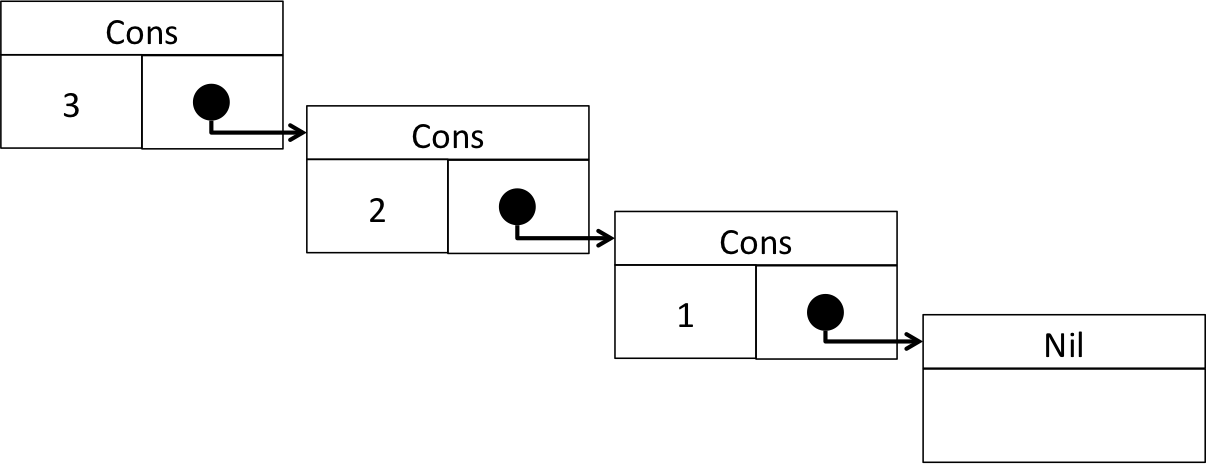
\includegraphics[scale=0.5]{linkedlist.png}
  \end{frame}

  \begin{frame}[fragile]
    \frametitle{Example 4: Vectors}
    Implement \texttt{Vec} like a linked list:
    \begin{minted}{csharp}
abstract class Vec<N, T> { }
sealed class Nil<T> : Vec<Z, T> { }
sealed class Cons<N, T> : Vec<S<N>, T>
{
    public T Head { get; private set; }
    public Vec<N, T> Tail { get; private set; }
    public Cons(T elem, Vec<N, T> tail)
    {
        Head = elem;
        Tail = tail;
    }
}
    \end{minted}
\end{frame}

  \begin{frame}[fragile]
    \frametitle{Example 4: Vectors}
    \begin{minted}{csharp}
static class VecExtensions
{
    public static T First<N, T>(this Vec<S<N>, T> v)
    {
        return ((Cons<N, T>)v).Head;  // :(
    }
    public static T Single<T>(this Vec<S<Z>, T> v)
    {
        return v.First();
    }
}
    \end{minted}
    
    We know that the only way to get a \texttt{Vec} longer than 0 is if it's a \texttt{Cons},
    but the language can't assume that because subclassing is \emph{open}.
    You're forced to squeeze your ideas into an unsuitable subtyping relationship.
\end{frame}

  \begin{frame}[fragile]
    \frametitle{Problems}
    Annoying to manually specify all your types:
    \begin{minted}{csharp}
var v = new Cons<S<S<Z>>, int>(2,
    new Cons<S<Z>, int>(3,
        new Cons<Z, int>(7, new Nil<int>())
    )
);
    \end{minted}
    
    \pause
    
    Luckily C$\sharp$ does (some) type inference of generic methods:
    
    \begin{minted}{csharp}
static Vec<S<N>, T> Cons<N, T>(T x, Vec<N, T> v)
{
    return new Cons<N, T>(x, v);
}
Cons(2, Cons(3, Cons(7, new Nil<int>()));
    \end{minted}
\end{frame}

  \begin{frame}[fragile]
    \frametitle{More problems}
    \textbf{Problem}: You can build a vector but you can't consume one ---
    C$\sharp$ is too dumb to infer the type of the tail of a vector.
    
    \begin{minted}{csharp}
public static int Sum(Vec<Z, int> v)
{
    return 0;
}
public static int Sum<N>(Vec<S<N>, int> v)
{
    var c1 = (Cons<N, int>)v;
                  // compile failure :(
    return c1.Head + Sum(c1.Tail);
}
Sum(Cons(2, Cons(3, new Nil<int>())));
    \end{minted}
\end{frame}

  \begin{frame}[fragile]
    \frametitle{99 problems but a Vec ain't one. Actually that's not true}
    Type syonyms would be useful
    \begin{minted}{csharp}
class Three : S<S<S<Z>>> { }
class Four : S<Three> { }  // not the same as S<S<S<S<Z>>>>
    \end{minted}
    
    No way to teach the type checker how to manipulate numbers - \emph{you can't compute with types}.
    \begin{minted}{csharp}
Vec</* Plus<N, M>? */, T> Extend<N, M, T>(
    Vec<N, T> v1,
    Vec<M, T> v2)

Vec<N, T> Take<N, M, T>(N length, Vec<M, T> v2)
    // where LEq<N, M>?
    \end{minted}
\end{frame}

  \begin{frame}
    \centering
    
\includegraphics[scale=0.3]{brain_melt_1.jpg}
  \end{frame}

  \begin{frame}[fragile]
    \frametitle{Here's what you could've won}
    \begin{minted}{idris}
data Vect : Nat -> Type -> Type where
    Nil : Vect Z a
    (::) : a -> Vect n a -> Vect (S n) a

head : Vect (S n) a -> a
head (x :: xs) = x

sum : Vect n Int -> Int
sum Nil = 0
sum (x :: xs) = x + sum xs

(++) : Vect n a -> Vect m a -> Vect (n + m) a
(++) Nil ys = ys
(++) (x :: xs) ys = x :: extend xs ys

take : n -> Vect (n + m) a -> Vect n a
take Z xs = Nil
take (S k) (x :: xs) = x :: take k xs
    \end{minted}
\end{frame}
  
  \begin{frame}
    \frametitle{The End}
    \begin{columns}
    \column{0.6\textwidth}
      \begin{itemize}
        \item Types can be part of your arsenal in the battle against bugs
        \item Generics give you a lot of generality and type-safety at little expense
        \item C$\sharp$ has plenty of room for improvement. I would like to see at least some of:
        \begin{itemize}
          \item Variant classes
          \item Anonymous subclasses
          \item Proper type inference
          \item Closed types and pattern matching
          \item Type syonyms
          \item Higher-kinded types
          \item Type functions
        \end{itemize}
        \item I've barely scratched the surface of crazy type systems available in today's programming languages
      \end{itemize}
    \column{0.4\textwidth}
      
\includegraphics[scale=0.25]{keanu.jpg}
    \end{columns}
  \end{frame}
\end{document}